\documentclass[abstract=on]{scrartcl}

\usepackage{textcomp}
\usepackage{filecontents}
\usepackage{eurosym}
\usepackage{natbib}
\usepackage{array}
\usepackage{setspace}
\usepackage{tabu}
\usepackage{adjustbox}
\usepackage{graphicx,epstopdf}
\usepackage[final]{pdfpages}
\usepackage[margin=1in]{geometry}
\usepackage[hidelinks]{hyperref}
\usepackage{booktabs}
\usepackage{tabularx}
\usepackage{floatrow}
\usepackage{amsmath}
\usepackage{amssymb}
\usepackage{float}
\restylefloat{table}
\usepackage{floatrow}
\usepackage{longtable}
\floatsetup[table]{capposition=top}
\floatsetup[figure]{capposition=top}
\usepackage{verbatim}
\bibliographystyle{spbasic}
\begin{document}
\date{}

\title{
Still learning to catch-up?\\
Technological capabilities, globalisation and economic growth\\
Supplementary appendix\thanks{The authors gratefully acknowledge funding by the Oesterreichische Nationalbank (OeNB,  Anniversary Fund, project number: 18144).}
}

% \titlerunning{}        
% \titlerunning{}        

\maketitle
\begin{abstract}
First, the supplementary material introduces and discusses the index of economic complexity, which we use to proxy for technological capabilities. Second, we list the countries included in the country sample. Third, we present descriptive statistics. Fourth, we report additional regression results when using an alternative proxy for institutional quality. Fifth, we show residual plots and diagnostics for the main econometric models estimates in the paper. Finally, we show a matrix with pair-wise correlations of relevant variables.
\end{abstract}

\newpage

\appendix

\newpage
\section{The economic complexity index}
\label{ap:eci}
The index of economic complexity (ECI) was first introduced in \citet{Hidalgo:2007cp} and further explicated in \citet{Hidalgo:2009be} and \citet{Hausmann:2013vj}.
For the underlying theory and a further interpretation, according to which the fundamental driving force for the development of nations is their ability to accumulate more and more information, see \citet{TheEconomicComplex:2011tp} and \citet{Hidalgo:2015vs}.

The index can be understood as a measure of the knowledge intensity of an economy, or, in other words, the amount of technological capabilities present in this economy. 
Its prominence stems from the fact that it is an excellent predictor for future growth rates of national economies, indicating that ``countries tend to approach the levels of income that correspond to their measured complexity`` \citep[p. 10574]{Hidalgo:2009be}.
% Interestingly, a similar link was suggested for income inequality \citep{Hartmann:2017ic}.
Here, we will briefly illustrate the way in which the indicator is constructed in the database we use \citep{TheEconomicComplex:2011tp}.
For a criticism of the computation method and an alternative see \citet{Cristelli:2013hj}.

\subsection{The computation of the index via the method of reflections}

One first needs to compute the \textit{revealed competitive advantage} (RCA) of each country $c$ with regard to every product $p$.
The $RCA_{cp}$ is constructed by asking whether the share of a product in the export basket of a country is smaller or larger than the share of this product in the total exports of the world market as a whole.
In other words, assuming that $P$ is the set of all products and $C$ the set of all countries, one relates the share of product $p\in P$ in the export basket of country $c\in C$, $\frac{X_{cp}}{\sum_{p'\in P}X_{cp'}}$, to the share of the product in total exports in the world, $\frac{\sum_{c'\in C}X_{c'p}}{\sum_{c'\in C}\sum_{p'\in P}X_{c'p'}}$.
Thus, the $RCA$ of country $c$ in product $p$ is given by:

\begin{align}
RCA_{cp}&=\frac{X_{cp} / \sum_{p'\in P}X_{cp'}}{\sum_{c'\in C}X_{c'p}/\sum_{c'\in C}\sum_{p'\in P}X_{c'p'}}
\end{align}

If $RCA_{cp}>1$ one says that country $c$ has a revealed comparative advantage in a product $p$.

Based on the $RCA$ one can construct a bipartite network of countries and products in which a country $c$ is connected to a product $p$ if $RCA_{cp}>1$. 
The resulting network can be represented by the adjacency matrix $M_{cp}$.
For every single element $m_{cp}\in M_{cp}$ we have $m_{cp} = 1$ iff $RCA_{cp}>1$ and zero otherwise.
Consequently, the row sum of this matrix $\sum_pM_{cp}$ represents the diversity of a country's export basket, i.e. the number of different products the country exports with revealed competitive advantage, denoted by $k_{c,0}$.
The column sums, $\sum_cM_{cp}$, then are the ubiquity of a product, i.e. the number of countries that export a given product with revealed competitive advantage, denoted by $\kappa_{p,0}$.

The intuition now is to say that the fact that a country exports a very ubiquitous product carries little information about the stock of technological capabilities of this country:
if many other countries can produce this product as well, there cannot be anything special about it.
To illustrate the basic intuition, \citet{Hidalgo:2009be} use an analogy to Lego pieces:
if a child shows you a very simplistic Lego building that could be built from almost any set of Lego pieces, it is hard to infer the stock of Lego pieces owned by that child.
Yet, when a country exports a product that is only produced by few other countries, this seems to be something special.
This corresponds to a child that provides you with a Lego building that requires very specific Lego pieces. 
After having seen the building, you can be very sure that the child possesses these specific pieces.

The same reasoning can be applied to the complexity of products :
if a product is exported by almost all countries, the product is probably not very complex -- it does not seem to require many capabilities. 
Yet, when there are only few countries exporting the product, then the product seems to be rather special.
Or, in terms of the Lego analogy:
if every child can build a certain building, it does not require particularly sophisticated pieces.
Yet, if only very few children can make the building, the required pieces are probably rare and difficult to acquire.

This intuitive logic can be expressed in terms of  $M_{cp}$.
As indicated above

\begin{align}
k_{c,0} &= \sum_pM_{cp} = \text{Diversity of export basket}\\
\kappa_{p,0} &= \sum_cM_{cp} = \text{Ubiquity of the product}
\end{align}

but this does not take into account the information that a less ubiquitous product carries more information about the capabilities of a country than an ubiquitous one.
Similarly, we would like to consider the complexity of a country for the calculation of the complexity of a product.
For example, for the complexity of countries we would like to take into account the average ubiquity of the products they export, but also the average diversity of the countries that export these products since this information is important to determine the general ubiquity of a product.
It is easy to see that this gives rise to a recursion of the following form:

\begin{align}
\label{eq:req-c}
k_{c,N} &= \frac{1}{k_{c,0}} \sum_pM_{cp} \kappa_{p,N-1} \\
\label{eq:req-p}
\kappa_{p,N} &= \frac{1}{\kappa_{p,0}} \sum_cM_{cp} k_{c,N-1}
\end{align}

Because $k_{c,N}$ and $\kappa_{p,N}$ are related to each other, the whole procedure has been termed `method of reflections' \citep{Hausmann:2013vj}.
Since the following steps are equivalent for country and product complexity, we illustrate the procedure for country complexity only.
First we insert the equation, resulting in:
\begin{align}
k_{c,N} &= \frac{1}{k_{c,0}} \sum_pM_{cp} \frac{1}{\kappa_{p,0}} \sum_{c'}M_{c'p} k_{c',N-2} 
\end{align}

which can be simplified by rearranging the sum to:

\begin{align}
k_{c,N} &= \sum_{c'} k_{c',N-2}   \sum\frac{M_{cp} M_{c'p}}{k_{c,0} \kappa_{p,0}}. 
\end{align}

Setting $\tilde{M}_{cc'}=\sum_p\frac{M_{cp} M_{c'p}}{k_{c,0} \kappa_{p,0}} $ we get

\begin{align}
k_{c,N} &= \sum_{c'} k_{c',N-2}   \tilde{M}_{cc'}.\label{eq:final-rec-c}
\end{align}

The recursion \eqref{eq:final-rec-c} reaches an equilibrium whenever $k_{c,N}=k_{c,N-2}=1$.
Taking the eigenvector $\vec{K}$ that corresponds to the second-largest eigenvalue of $\tilde{M}_{cc'}$ in equilibrium yields the index of economic complexity ECI, which we first normalize by its mean and standard deviation:\footnote{Why not taking the eigenvector that corresponds to the largest eigenvalue of $\tilde{M}_{cc'}$ in equilibrium? 
It is easy to show that this eigenvector necessarily consists only of ones.
Since we are interested in the differences among countries, it is the second-largest eigenvector that carries most of the relevant information.}

\begin{align}
ECI=\frac{\vec{K}-mean(\vec{K})}{sd(\vec{K})}
\end{align}

The product complexities $PCI$ are obtained in exactly the same way.
Assuming that $\vec{Q}$ is the product equivalent to $\vec{K}$ then $PCI$ is obtained via:

\begin{align}
PCI=\frac{\vec{Q}-mean(\vec{Q})}{sd(\vec{Q})}
\end{align}

Hence, $PCI$ is a measure for the complexity of a product in the sense that complex products require many and very sophisticated capabilities to be produced, while simple products can be produced without such capabilities.
$ECI$ is a measure for the knowledge intensity of an economy, or the amount of available technological capabilities.
The more complex a country, the more capabilities it has and the more complex products it can produce:
just as one can infer the presence of particular Lego pieces by the buildings a child was able to built, one can infer the presence of particular capabilities by looking at the products a country is able to export \citep{Hidalgo:2009be}.

Empirically, we can observe that more complex countries have more diversified export baskets \citep[they do not necessarily stop exporting simple products, see][]{Tacchella:2013ko}, enjoy higher levels of income \citep{Hidalgo:2009be} and lower levels of income inequality \citep{Hartmann:2017ic}.

% Because of the mutual dependence of country and product complexity, countries that export rare raw materials, such as oil, do not necessarily enjoy high complexity, since the raw material gets penalized...

The method of reflections has been criticized by \citet{Tacchella:2013ko}, who suggest an alternative computation method. 
The resulting ranking is slightly different, in particular for developing countries.
See \citet{Tacchella:2012fx} and \citet{Tacchella:2013ko}  for further details and a thorough comparison.

\subsection{Strengths and weaknesses}
Although we believe that the ECI is an excellent analytical tool to study economic development, there are a number of drawbacks that we wish to point out:

\paragraph{Ambiguity with regard to the concept of `capabilities'}
Although this is not a particular weakness of the indicator as such, it should be mentioned that it does not contain any information on how capabilities have been acquired.
Furthermore, there is no full-fledged theory of capabilities backing the indicator.
It is clear that the capabilities include diverse aspects such as human and physical capital, national institutions, organizational capacities to coordinate diverse teams of people, and working practices and know-how on the firm level  \citep[e.g.][p. 37]{Felipe:2012fv}.
Additionally, it is recognized that capabilities come in both embodied and disembodied form, in tacit and codified versions, and that they relate both to the creation and dissemination of knowledge \citep[e.g.][p. 177-178]{Archibugi:2005iu}.
Yet, there is no specific theory about how these capabilities yield overall prosperity, although \citet{Hidalgo:2015vs} sketches a theory based on ``person bytes'', which has, however, not (yet) been discussed widely in the scientific community.

\paragraph{No distinction between technological and productive capabilities}
A potential drawback of the ECI is that it does not distinguish between technological and productive capabilities as suggested in, among others, \citet[p. 919]{Archibugi:2009bf}. 
Such a distinction can be useful if one wishes to study how an increase of technological capabilities impacts on the productive capabilities of an economy. 
However, this distinction is often hard to make in practice since the production process itself usually impacts on technological capabilities (e.g. via \textit{learning by doing}).
Also, as argued in \citet{Hidalgo:2015vs}, products can be seen as a `crystalized' form of technological capabilities.
As long as one is not concerned with very specific questions on the relationship between a country's ability to produce goods and its level of technological capabilities, the distinction does not seem to be decisive.

%\paragraph{Distortions for advanced resource-rich countries}
%In general, the method of reflections does a good job in handling ressource-rich economies: 
%although only few countries export, say, raw oil, these countries do receive a higher complexity score if they do not export other complex products:
%since raw oil is exported mainly by developing countries, it is -- even only few countries export it -- not a complex product.
%Yet, there are always some special cases, such as Norway (which has, due to the extensive export of raw materials, a rather low complexity) or \textbf{XXX}.

\paragraph{Measurement problems}
Since the indicator is built using trade data it inhabits all methodological and measurement problems associated with trade data. 
For example, the SITC codes used for long-term evolution of the ECI have problems in accommodating new products, such as smartphones.
The more accurate harmonized system (HS) also experiences some problems: in 2007, for example, the new 2007 version of the HS system has been released. 
Some older categories still present in the 1992 version were dropped and integrated into other product codes.
Some countries stopped reporting such products in the HS92 version of the system as well.
This has lead to an apparent drop in the production of some products, and a corresponding rise in complexity for, e.g. tin products.
The best way to avoid this problem is to use the most recent version of the HS system - yet this inevitably comes with a loss in data coverage.

\paragraph{Lack of services} 
Another negative side-effect of the reliance on trade data is the lack of services:
since trades in services do not pass custom offices, not all countries report service flows. 
Consequently, building the complexity index for services would necessarily yield results biased in favour of countries declaring services.
Thus, a country's complexity takes into account only real products. 
This might be a problem for countries that rely heavily on services, or that have experienced strong de-industrialization.\\

Despite these drawbacks, we believe that the ECI is a very useful tool to study economic development. 
Among its many advantages we would like to stress the following:

\paragraph{Outcome-based measure}
The ECI is an outcome-based measure, i.e. it directly measures what countries make of their situation, rather than considering their institutional or geographical conditions with regard to their benefit for technological change.
This facilitates cross-country comparisons compared to composite indicators based on institutional data:
a law that works in one country does not necessarily work in another, which is why a comparison of countries in terms of their legal frameworks can be misleading if one is ultimately interested in their technological capabilities.
Comparing the capabilities directly is probably a better choice.

\paragraph{Excellent coverage}
Since the ECI is calculated from trade data it is available for almost all UN countries from 1963. 
This exceeds the coverage of many alternatives by magnitudes and allows for promising long-run investigations.

\paragraph{Few degrees of freedom} 
Many composite indicators aggregate the information from various sources.
During the aggregation procedure, the various ingredients usually get weighted -- a source of subjectivity and variation.
For the ECI, on the other hand, there are not many ways to compute it.
In fact, aside from the 'method of reflections' we are aware only of the alternative method of \citet{Tacchella:2013ko} to derive the index.

\paragraph{Intuitive interpretation and good predictor for economic growth}
The interpretation of the ECI is straightforward.
Complex countries have many and sophisticated capabilities.
They tend to be rich because they can transform inputs to outputs in fancy ways.
Less complex products do not have these capabilities, which is why they are less developed.
Also, the complexity and relatedness of products can be illustrated very nicely through the \textit{product space} \citep{Hidalgo:2007cp}.


\subsection{Related literature}
Here, we provide a very concise survey of the related literature and mention some related indices.
The interested reader might refer to these sources for further information on the corresponding indices and concepts.

\subsubsection{Theoretical accounts of technological capabilities}
Although the ECI does not directly build upon a particular theory of capability accumulation, it suggests that the technological capabilities of a country are decisive for its future development.
The idea that capabilities are at the heart of economic development and should be of prime interest for directed policy intervention dates back to at least \citet{Hirschman:1958wr}, see also \citet{Lall:1992eq} or \citet{Bell:1995wj}.
Today, capabilities as determinants for economic development receive particular attention in the evolutionary literature on technological change \citep[see e.g.][]{Dosi:2015ug} and in the area of evolutionary economic geography \citep[e.g.][]{Boschma:2016kg}.

More directly, the ECI builds upon the work of \citet{Hausmann:2007hj}, who relate products to the level of income of the economies that export these products with a revealed competitive advantage.
They already call it `product complexity'. 
They also suggest a measure called `export complexity', which is related to the average product complexity of a countries' export basket.
Thus, the paper concludes that ``what you export matters'' for economic development \citep[p. 1]{Hausmann:2007hj}.
This idea then was the basis for the `product space' \citep{Hidalgo:2007cp}.
Here, the authors use export data to show that some products are important in the sense that they indicate the presence of capabilities that can be re-used in a variety of ways, while other products are associated with capabilities that are much less useful and only help to produce few peripheral products.

The idea that a country has to accumulate a complete set of capabilities before it can produce a certain product has similarities to the `O-Ring' theory of development of \citet{Kremer:1993cs} 
He argues that the production of products involves different tasks, and once the knowledge has been required for one particular task, certain products cannot be produced at all. 
A similar argument is made by \citet{Sutton:2012uka}, although from a firm perspective.

\subsubsection{Related indices}
There are some related indices that might be viable alternatives to the ECI in some instances.
The most similar one is suggested by \citet{Tacchella:2012fx, Tacchella:2013ko}.
From the underlying intuition, it is quasi-equivalent to the original ECI, yet the computation method is slightly different -- and so is the resulting ranking.
The differences are most pronounced for developing countries, see \citet{Cristelli:2013hj} for a more detailed comparison.

Furthermore, a number of other indicators for technological capabilities have been used in the literature, e.g.
the Technology index of \citet{Furman:2002gu}, which has been integrated to the WEF Global Competitive Report,  
the \textit{AcCo Index} by \citet{Archibugi:2004bp},
the \textit{Science and Technology Capacity Index} of \citet{Wagner:2001up}, and
the \textit{innovation index} by \citet{Khayyat:2015ks}.

Most of these measures are surveyed and compared in \citet{Archibugi:2005iu} and more recently in \citet{Archibugi:2009bf} and \citet{Felipe:2012fv}.
They are mainly composite indices that aggregate a number of different variables measuring the innovative capacities of economies such as \textit{patents per million population}, \textit{R\&D expenditure}, \textit{schooling} and \textit{use of computers}.
Thus, they are not directly output-oriented such as the ECI but rather concerned with the conditions necessary for positive technological change.\footnote{A similar approach for the classification of products is undertaking by the complex products and system (CoPS) category of \citet{Hobday:2000hx}. The latter, however, also takes a broader range of inputs into consideration.}
This way, they approach the problem of measuring technological capabilities in a different way than the ECI, which does not rely on any aggregation, but directly measures the outcome of technological capability building.
Thus, they might be preferable if one seeks to study the conditions required for the accumulation of technological capabilities, but not so much the capabilities as such.

Finally, note that since the ECI is computed directly from import-export data, which is readily available for a vast majority of countries, its time and country coverage is much higher than that of the alternative indicators.

\section{Data sample}

The 108 countries included in the econometric analysis are: Albania, Argentina, Australia, Austria, Burundi, Belgium, Benin, Burkina Faso, Bulgaria, Bolivia, Brazil, Barbados, Central African Republic, Canada, Switzerland, Chile, China, Cote d’Ivoire, Cameroon, Congo, Colombia, Costa Rica, Cyprus, Germany, Denmark, Dominican Republic, Algeria, Ecuador, Egypt, Spain, Ethiopia, Finland, Fiji, France, Gabon, United Kingdom, Ghana, Gambia, Greece, Guatemala, Hong Kong SAR China, Honduras, Haiti, Hungary, Indonesia, India, Ireland, Iraq, Iceland, Israel, Italy, Jamaica, Jordan, Japan, Kenya, Cambodia, South Korea, Kuwait, Laos, Liberia, Morocco, Madagascar, Maldives, Mexico, Mali, Malta, Myanmar (Burma), Mongolia, Mauritania, Mauritius, Malawi, Malaysia, Niger, Nigeria, Nicaragua, Netherlands, Norway, Nepal, New Zealand, Pakistan, Panama, Peru, Philippines, Poland, Portugal, Paraguay, Rwanda, Saudi Arabia, Sudan, Senegal, Singapore, Sierra Leone, El Salvador, Sweden, Syria, Togo, Thailand, Trinidad and Tobago, Tunisia, Turkey, Tanzania, Uganda, Uruguay, United States of America, Venezuela, Vietnam, South Africa, Zambia.

\section{Descriptive statistics}

Here are the descriptive statistics for the variables used in the econometric analysis.

\begin{table}[!htbp] \centering 
  \caption{Cross-sectional data (1985-2014)} 
  \label{} 

% Table created by stargazer v.5.2 by Marek Hlavac, Harvard University. E-mail: hlavac at fas.harvard.edu
% Date and time: Fri, Jan 21, 2022 - 19:14:49
\begin{tabular}{@{\hspace{5pt}}lccccc} 
\toprule 
 
Statistic & \multicolumn{1}{c}{N} & \multicolumn{1}{c}{Mean} & \multicolumn{1}{c}{St. Dev.} & \multicolumn{1}{c}{Min} & \multicolumn{1}{c}{Max} \\ 
\midrule \\[-2.1ex] 
eci & 108 & $-$0.007 & 1.035 & $-$2.336 & 2.410 \\ 
GDP\_pc\_PPP\_log & 108 & 8.480 & 1.106 & 6.658 & 10.404 \\ 
AdvancedCountry & 108 & 0.241 & 0.430 & 0 & 1 \\ 
HighIncome & 105 & 0.571 & 0.497 & 0 & 1 \\ 
LowIncome & 105 & 0.019 & 0.137 & 0 & 1 \\ 
LowerMiddleIncome & 105 & 0.181 & 0.387 & 0 & 1 \\ 
HigherMiddleIncome & 105 & 0.229 & 0.422 & 0 & 1 \\ 
OPECdummy & 108 & 0.074 & 0.263 & 0 & 1 \\ 
popgrowth & 108 & 1.687 & 1.014 & $-$0.718 & 4.078 \\ 
humancapital & 108 & 2.242 & 0.670 & 1.089 & 3.565 \\ 
primaryexports & 108 & 0.248 & 0.194 & 0.007 & 0.859 \\ 
oilexports & 108 & 12.346 & 22.294 & 0.023 & 95.417 \\ 
coalandmetalexports & 108 & 7.397 & 11.432 & 0.116 & 69.771 \\ 
avg\_GDP\_pc\_PPP\_growth & 108 & 2.463 & 1.751 & $-$1.950 & 7.187 \\ 
kof\_econ & 108 & 52.274 & 15.616 & 21.917 & 91.224 \\ 
inv\_share & 108 & 20.526 & 7.012 & 7.268 & 44.177 \\ 
domesticcredit & 108 & 47.401 & 41.663 & 3.811 & 197.284 \\ 
\bottomrule 
\end{tabular} 

\floatfoot{log(GDPpc)… logarithm of GDP per capita; ECI… Economic Complexity Index; global… KOF economic globalization index; pop… population growth; hc… human capital index; findev... financial development; oil… oil exports; coal… coal and metal exports. For more details on the variables see Table 1.
}
\end{table} 

\begin{table}[!htbp] \centering 
  \caption{Cross-sectional data (1990-2010)} 
  \label{} 

% Table created by stargazer v.5.2 by Marek Hlavac, Harvard University. E-mail: hlavac at fas.harvard.edu
% Date and time: Fri, Jan 21, 2022 - 19:14:49
\begin{tabular}{@{\hspace{5pt}}lccccc} 
\toprule 
 
Statistic & \multicolumn{1}{c}{N} & \multicolumn{1}{c}{Mean} & \multicolumn{1}{c}{St. Dev.} & \multicolumn{1}{c}{Min} & \multicolumn{1}{c}{Max} \\ 
\midrule \\[-2.1ex] 
eci & 89 & 0.050 & 1.096 & $-$2.126 & 2.639 \\ 
GDP\_pc\_PPP\_log & 89 & 8.629 & 1.172 & 6.625 & 10.516 \\ 
AdvancedCountry & 89 & 0.258 & 0.440 & 0 & 1 \\ 
HighIncome & 88 & 0.614 & 0.490 & 0 & 1 \\ 
LowIncome & 88 & 0.000 & 0.000 & 0 & 0 \\ 
LowerMiddleIncome & 88 & 0.170 & 0.378 & 0 & 1 \\ 
HigherMiddleIncome & 88 & 0.216 & 0.414 & 0 & 1 \\ 
OPECdummy & 89 & 0.079 & 0.271 & 0 & 1 \\ 
inv\_share & 89 & 18.972 & 10.356 & 1.751 & 45.460 \\ 
popgrowth & 89 & 1.591 & 1.010 & $-$0.869 & 3.568 \\ 
humancapital & 89 & 2.338 & 0.663 & 1.084 & 3.574 \\ 
primaryexports & 89 & 0.224 & 0.182 & 0.005 & 0.804 \\ 
oilexports & 89 & 12.559 & 22.339 & 0.030 & 91.644 \\ 
coalandmetalexports & 89 & 6.636 & 11.118 & 0.232 & 67.482 \\ 
avg\_GDP\_pc\_PPP\_growth & 89 & 2.856 & 1.935 & $-$1.720 & 8.594 \\ 
kof\_econ & 89 & 54.186 & 15.185 & 23.259 & 90.867 \\ 
politicalquality & 89 & 0.171 & 0.948 & $-$1.848 & 1.810 \\ 
economicquality & 89 & $-$0.037 & 0.899 & $-$2.145 & 1.624 \\ 
legalquality & 89 & 0.017 & 0.908 & $-$1.412 & 1.708 \\ 
propertyrights & 89 & 54.671 & 22.226 & 10.000 & 90.667 \\ 
domesticcredit & 89 & 48.924 & 41.388 & 3.461 & 176.142 \\ 
\bottomrule 
\end{tabular} 

\floatfoot{log(GDPpc)… logarithm of GDP per capita; ECI… Economic Complexity Index; global… KOF economic globalization index; pop… population growth; hc… human capital index; oil… oil exports; coal… coal and metal exports; einst… economic institutional quality; pinst… political institutional quality; linst… legal institutional quality. For more details on the variables see Table 1.
}
\end{table} 

\begin{table}[H] \centering 
  \caption{Panel data: 5-year averages (1985-2014)} 
  \label{} 

% Table created by stargazer v.5.2 by Marek Hlavac, Harvard University. E-mail: hlavac at fas.harvard.edu
% Date and time: Fri, Jan 21, 2022 - 19:14:50
\begin{tabular}{@{\hspace{5pt}}lccccc} 
\toprule 
 
Statistic & \multicolumn{1}{c}{N} & \multicolumn{1}{c}{Mean} & \multicolumn{1}{c}{St. Dev.} & \multicolumn{1}{c}{Min} & \multicolumn{1}{c}{Max} \\ 
\midrule \\[-2.1ex] 
eci & 756 & $-$0.051 & 1.056 & $-$2.773 & 2.936 \\ 
Penn\_GDP\_PPP\_log & 756 & 8.741 & 1.252 & 5.485 & 11.310 \\ 
GDP\_pc\_growth & 755 & 2.183 & 4.391 & $-$17.202 & 22.401 \\ 
kof\_econ & 756 & 51.577 & 17.038 & 14.720 & 93.187 \\ 
AdvancedCountry & 756 & 0.241 & 0.428 & 0 & 1 \\ 
HighIncome & 747 & 0.570 & 0.495 & 0 & 1 \\ 
LowIncome & 747 & 0.019 & 0.136 & 0 & 1 \\ 
LowerMiddleIncome & 747 & 0.185 & 0.388 & 0 & 1 \\ 
HigherMiddleIncome & 747 & 0.226 & 0.419 & 0 & 1 \\ 
popgrowth & 756 & 1.712 & 1.208 & $-$3.987 & 6.603 \\ 
humancapital & 756 & 2.216 & 0.695 & 1.022 & 3.723 \\ 
OPECdummy & 756 & 0.074 & 0.262 & 0 & 1 \\ 
inv\_share & 756 & 20.402 & 8.892 & 0.995 & 59.973 \\ 
\bottomrule 
\end{tabular} 

\floatfoot{log(GDPpc)… logarithm of GDP per capita; ECI… Economic Complexity Index; global… KOF economic globalization index; pop… population growth; hc… human capital index. For more details on data sources and variable descriptions see Table 1 in the main text.
}
\end{table} 

\newpage
\section{Additional regression results using an alternative proxy for institutional quality}

Columns (1) and (2) of the table below show the same results as in columns (7) and (9) of Table 3 in the main paper, respectively. Columns (3) and (4) of the table below show additional regressions results when we use a property rights index to proxy for institutional quality. 

\begin{table}[H] \centering 
\begin{tiny}
  \caption{} 
  \label{} 
  
% Table created by stargazer v.5.2 by Marek Hlavac, Harvard University. E-mail: hlavac at fas.harvard.edu
% Date and time: Fri, Jan 21, 2022 - 19:14:50
\begin{tabular}{@{\hspace{5pt}}l@{\hspace{5pt}}cccc} 
\toprule 
 & (1) & (2) & (3) & (4)\\ 
\midrule  
\\[-2.1ex] GDPpc (log) & $-$1.098$^{**}$ & $-$1.494$^{***}$ & $-$1.300$^{***}$ & $-$1.854$^{***}$ \\ 
  & (0.432) & (0.504) & (0.460) & (0.447) \\ 
 \addlinespace 
 Globalization & 0.047$^{**}$ & 0.046$^{*}$ & 0.032 & 0.032 \\ 
  & (0.024) & (0.024) & (0.022) & (0.021) \\ 
 \addlinespace 
 ECI & 5.947$^{***}$ & 6.642$^{***}$ & 6.183$^{***}$ & 7.140$^{***}$ \\ 
  & (1.937) & (2.170) & (1.890) & (2.049) \\ 
 \addlinespace 
 Political inst & $-$0.931 & $-$0.576 &  &  \\ 
  & (0.562) & (0.660) &  &  \\ 
 \addlinespace 
 Property rights &  &  & 0.011 & 0.021 \\ 
  &  &  & (0.021) & (0.020) \\ 
 \addlinespace 
 Population growth & $-$0.585$^{*}$ & $-$0.626$^{*}$ & $-$0.568$^{*}$ & $-$0.693$^{**}$ \\ 
  & (0.334) & (0.334) & (0.308) & (0.303) \\ 
 \addlinespace 
 Human capital & 1.784$^{***}$ & 1.747$^{***}$ & 1.262$^{**}$ & 1.370$^{***}$ \\ 
  & (0.510) & (0.523) & (0.505) & (0.499) \\ 
 \addlinespace 
 Oil exports &  & 0.020 &  & 0.028$^{**}$ \\ 
  &  & (0.012) &  & (0.011) \\ 
 \addlinespace 
 GDPpc (log) \cdot ECI & $-$0.653$^{***}$ & $-$0.705$^{***}$ & $-$0.707$^{***}$ & $-$0.772$^{***}$ \\ 
  & (0.194) & (0.214) & (0.192) & (0.204) \\ 
 \addlinespace 
 Constant & 7.316$^{*}$ & 10.699$^{**}$ & 10.365$^{***}$ & 14.230$^{***}$ \\ 
  & (3.869) & (4.607) & (3.632) & (3.491) \\ 
 \addlinespace 
\midrule  
Observations & 89 & 89 & 89 & 89 \\ 
R$^{2}$ & 0.323 & 0.351 & 0.284 & 0.351 \\ 
Adjusted R$^{2}$ & 0.264 & 0.286 & 0.223 & 0.286 \\ 
\bottomrule 
\textit{Note:}  & \multicolumn{4}{r}{$^{*}$p$<$0.1; $^{**}$p$<$0.05; $^{***}$p$<$0.01} \\ 
\end{tabular} 

  \begin{comment}
\begin{tabular}{@{\extracolsep{5pt}}lcccc} 
\\[-1.8ex]\hline 
\hline \\[-1.8ex] 
\\[-1.8ex] & (1) & (2) & (3) & (4)\\ 
\\[-1.8ex] & pinst & pinst + oil & prights & prights + oil\\ 
\hline \\[-1.8ex] 
 log(GDPpc) & $-$1.098$^{**}$ & $-$1.494$^{***}$ & $-$1.300$^{***}$ & $-$1.854$^{***}$ \\ 
  & (0.432) & (0.504) & (0.460) & (0.447) \\ 
  & & & & \\ 
 ECI & 5.947$^{***}$ & 6.642$^{***}$ & 6.183$^{***}$ & 7.140$^{***}$ \\ 
  & (1.937) & (2.170) & (1.890) & (2.049) \\ 
  & & & & \\ 
  global & 0.047$^{**}$ & 0.046$^{*}$ & 0.032 & 0.032 \\ 
  & (0.024) & (0.024) & (0.022) & (0.021) \\ 
  & & & & \\ 
  pop & $-$0.585$^{*}$ & $-$0.626$^{*}$ & $-$0.568$^{*}$ & $-$0.693$^{**}$ \\ 
  & (0.334) & (0.334) & (0.308) & (0.303) \\ 
  & & & & \\ 
 hc & 1.784$^{***}$ & 1.747$^{***}$ & 1.262$^{**}$ & 1.370$^{***}$ \\ 
  & (0.510) & (0.523) & (0.505) & (0.499) \\ 
  & & & & \\ 
 pinst & $-$0.931 & $-$0.576 &  &  \\ 
  & (0.562) & (0.660) &  &  \\ 
  & & & & \\ 
 prights &  &  & 0.011 & 0.021 \\ 
  &  &  & (0.021) & (0.020) \\ 
  & & & & \\ 
 oil &  & 0.020 &  & 0.028$^{**}$ \\ 
  &  & (0.012) &  & (0.011) \\ 
  & & & & \\ 
 log(GDPpc) $\cdot$ ECI & $-$0.653$^{***}$ & $-$0.705$^{***}$ & $-$0.707$^{***}$ & $-$0.772$^{***}$ \\ 
  & (0.194) & (0.214) & (0.192) & (0.204) \\ 
  & & & & \\ 
 Constant & 7.316$^{*}$ & 10.699$^{**}$ & 10.365$^{***}$ & 14.230$^{***}$ \\ 
  & (3.869) & (4.607) & (3.632) & (3.491) \\ 
  & & & & \\ 
\hline \\[-1.8ex] 
Observations & 89 & 89 & 89 & 89 \\ 
R$^{2}$ & 0.323 & 0.351 & 0.284 & 0.351 \\ 
\hline 
\hline \\[-1.8ex] 
\textit{Note:}  & \multicolumn{4}{r}{$^{*}$p$<$0.1; $^{**}$p$<$0.05; $^{***}$p$<$0.01} \\ 
\end{tabular} 
  \end{comment}
\end{tiny}
\end{table} 

\newpage
\section{Residual plots and diagnostics}

The following plots are based on model (6) in Table 1.

\begin{figure}[H]
 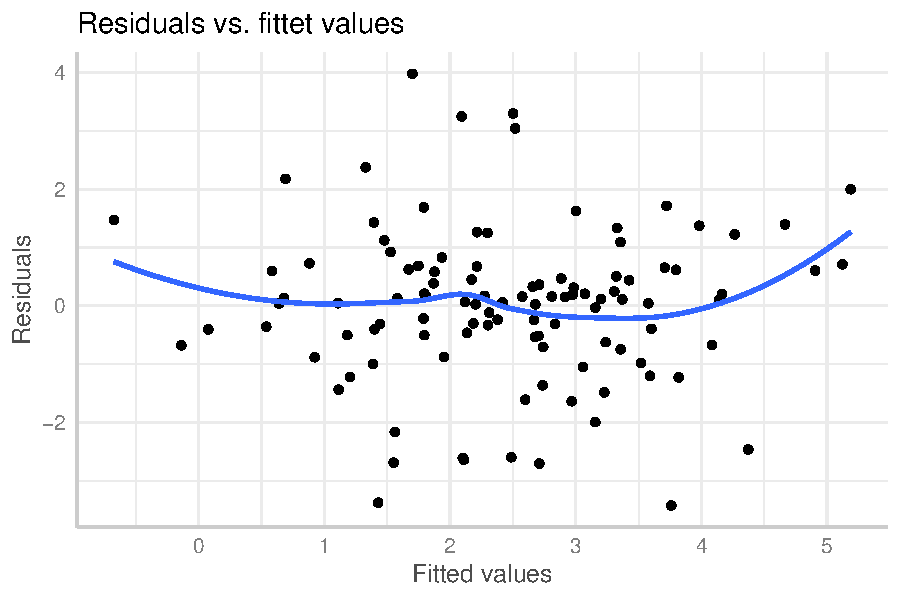
\includegraphics[width=0.6\textwidth, height=200px]{A5-ResidualPlot.pdf}
 \caption{Residuals vs. fitted values}
\label{Figure 3}
\end{figure}

\begin{figure}[H]
 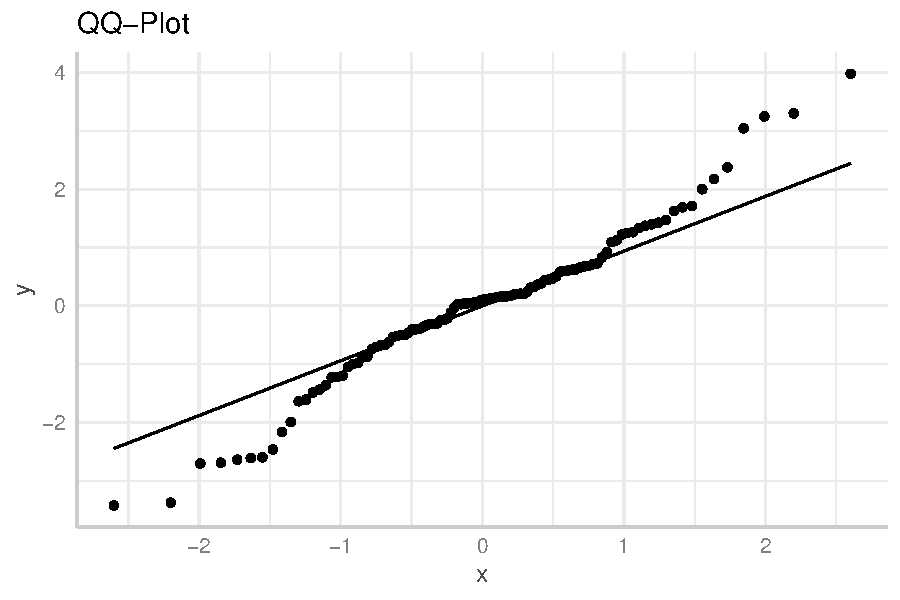
\includegraphics[width=0.6\textwidth, height=200px]{A6-QQPlot.pdf}
 \caption{Quantile-Quantile plot}
\label{Figure 3}
\end{figure}

Here is the result from the Durbin-Watson test on autocorrelation:

% latex table generated in R 4.1.2 by xtable 1.8-4 package
% Mon Mar 28 20:53:05 2022
\begin{table}[ht]
\centering
\begin{tabular}{rr}
  \toprule
DW & p-value \\ 
  \midrule
1.782 & 0.137 \\ 
   \bottomrule
\end{tabular}
\end{table}


\newpage

\section{Correlation matrix (Pearson correlation coefficients)}

Here are the pairwise-correlations of the variables based on Pearson correlation coefficients for the cross-sectional data of the time period 1990-2010.

% latex table generated in R 4.0.4 by xtable 1.8-4 package
% Fri Jan 21 19:14:50 2022
\begin{table}[ht]
\centering
\begin{tabular}{rrrrrrrrrrr}
  \toprule
 & ECI & GDPpc & growth & global & pop & hc & linst & pinst & einst & oil \\ 
  \midrule
ECI & 1.00 & 0.78 & 0.05 & 0.67 & -0.65 & 0.77 & 0.79 & 0.80 & 0.77 & -0.33 \\ 
  GDPpc & 0.78 & 1.00 & 0.01 & 0.77 & -0.58 & 0.86 & 0.82 & 0.82 & 0.84 & 0.01 \\ 
  growth & 0.05 & 0.01 & 1.00 & 0.09 & -0.25 & 0.16 & 0.01 & -0.01 & 0.08 & 0.07 \\ 
  global & 0.67 & 0.77 & 0.09 & 1.00 & -0.43 & 0.75 & 0.78 & 0.76 & 0.87 & -0.08 \\ 
  pop & -0.65 & -0.58 & -0.25 & -0.43 & 1.00 & -0.67 & -0.58 & -0.62 & -0.52 & 0.27 \\ 
  hc & 0.77 & 0.86 & 0.16 & 0.75 & -0.67 & 1.00 & 0.84 & 0.85 & 0.83 & -0.15 \\ 
  linst & 0.79 & 0.82 & 0.01 & 0.78 & -0.58 & 0.84 & 1.00 & 0.97 & 0.90 & -0.29 \\ 
  pinst & 0.80 & 0.82 & -0.01 & 0.76 & -0.62 & 0.85 & 0.97 & 1.00 & 0.90 & -0.32 \\ 
  einst & 0.77 & 0.84 & 0.08 & 0.87 & -0.52 & 0.83 & 0.90 & 0.90 & 1.00 & -0.27 \\ 
  oil & -0.33 & 0.01 & 0.07 & -0.08 & 0.27 & -0.15 & -0.29 & -0.32 & -0.27 & 1.00 \\ 
   \bottomrule
\end{tabular}
\end{table}

\begin{comment}

\begin{verbatim}
         ECI GDPpc growth global   pop    hc linst pinst einst   oil
ECI     1.00  0.78   0.05   0.67 -0.65  0.77  0.79  0.80  0.77 -0.33
GDPpc   0.78  1.00   0.01   0.77 -0.58  0.86  0.82  0.82  0.84  0.01
growth  0.05  0.01   1.00   0.09 -0.25  0.16  0.01 -0.01  0.08  0.07
global  0.67  0.77   0.09   1.00 -0.43  0.75  0.78  0.76  0.87 -0.08
pop    -0.65 -0.58  -0.25  -0.43  1.00 -0.67 -0.58 -0.62 -0.52  0.27
hc      0.77  0.86   0.16   0.75 -0.67  1.00  0.84  0.85  0.83 -0.15
linst   0.79  0.82   0.01   0.78 -0.58  0.84  1.00  0.97  0.90 -0.29
pinst   0.80  0.82  -0.01   0.76 -0.62  0.85  0.97  1.00  0.90 -0.32
einst   0.77  0.84   0.08   0.87 -0.52  0.83  0.90  0.90  1.00 -0.27
oil    -0.33  0.01   0.07  -0.08  0.27 -0.15 -0.29 -0.32 -0.27  1.00
\end{verbatim}
GDPpc… logarithm of GDP per capita; ECI… Economic Complexity Index; global… KOF economic globalization index; pop… population growth; hc… human capital index; oil… oil exports; coal… coal and metal exports; einst… economic institutional quality; pinst… political institutional quality; linst… legal institutional quality; oil: share of oil exports in total exports. For more details on the variables see Table 1 in the main text.
\end{comment}
\bibliography{cjebib}


\end{document}